\section{The Sosiogram}
During the project the facilitators went around to the groups, analyzing how the communication within the team was during a discussion. They made a sosiogram of it by dotting down lines whenever someone talked to individuals or the group as a whole, as we can see in the sosiogram from our group, seen in \autoref{fig:sosiogram}. Note that when someone talked to the group in general, it's represented as a line towards the center dot of the "table".



None of the group members knew that they were being facilitated. The interesting thing about this event was that every group member were surprised over the how the communication flow degenerated. Hanne was one of the most active in the group. She was surprised that she didn't notice that  Marius and Erik wasn’t participating in the discussion. She felt that all members were contributing. Marius was one of the members that were focused on doing research on the computer while the group had a meeting. He was also surprised over the sociogram because he felt that he could do research at the same time as contributing in the group meeting. 

From the sociogram the group reached the conclusion that the two people sitting on their laptop during the meeting, even though they were doing work relevant for the project, was much less active in the discussion. Since one of the big advantages of a group project is that you get different points of view and can have a discussion about the subject the group decided that this was something we didn't want. We wanted to see the effect of interdisciplinary backgrounds. Since the sociogram showed that everyone was about as active as the others, with exception of those using their laptop , we decided to add a norm saying that from now on every meeting shall be pc-free, unless someone was specifically asked to either take notes as a secretary, or check something that we would need in the discussion.

We managed to keep this norm for the rest of the project and we felt that it improved our creativity and productivity. It is hard to measure it, but the thing we noticed was that we didn't have to repeat the same topics that had been discussed earlier because all group members paid attention and focused on the meeting. 
\newpage{}
\begin{figure}
	\begin{center}
		\frame{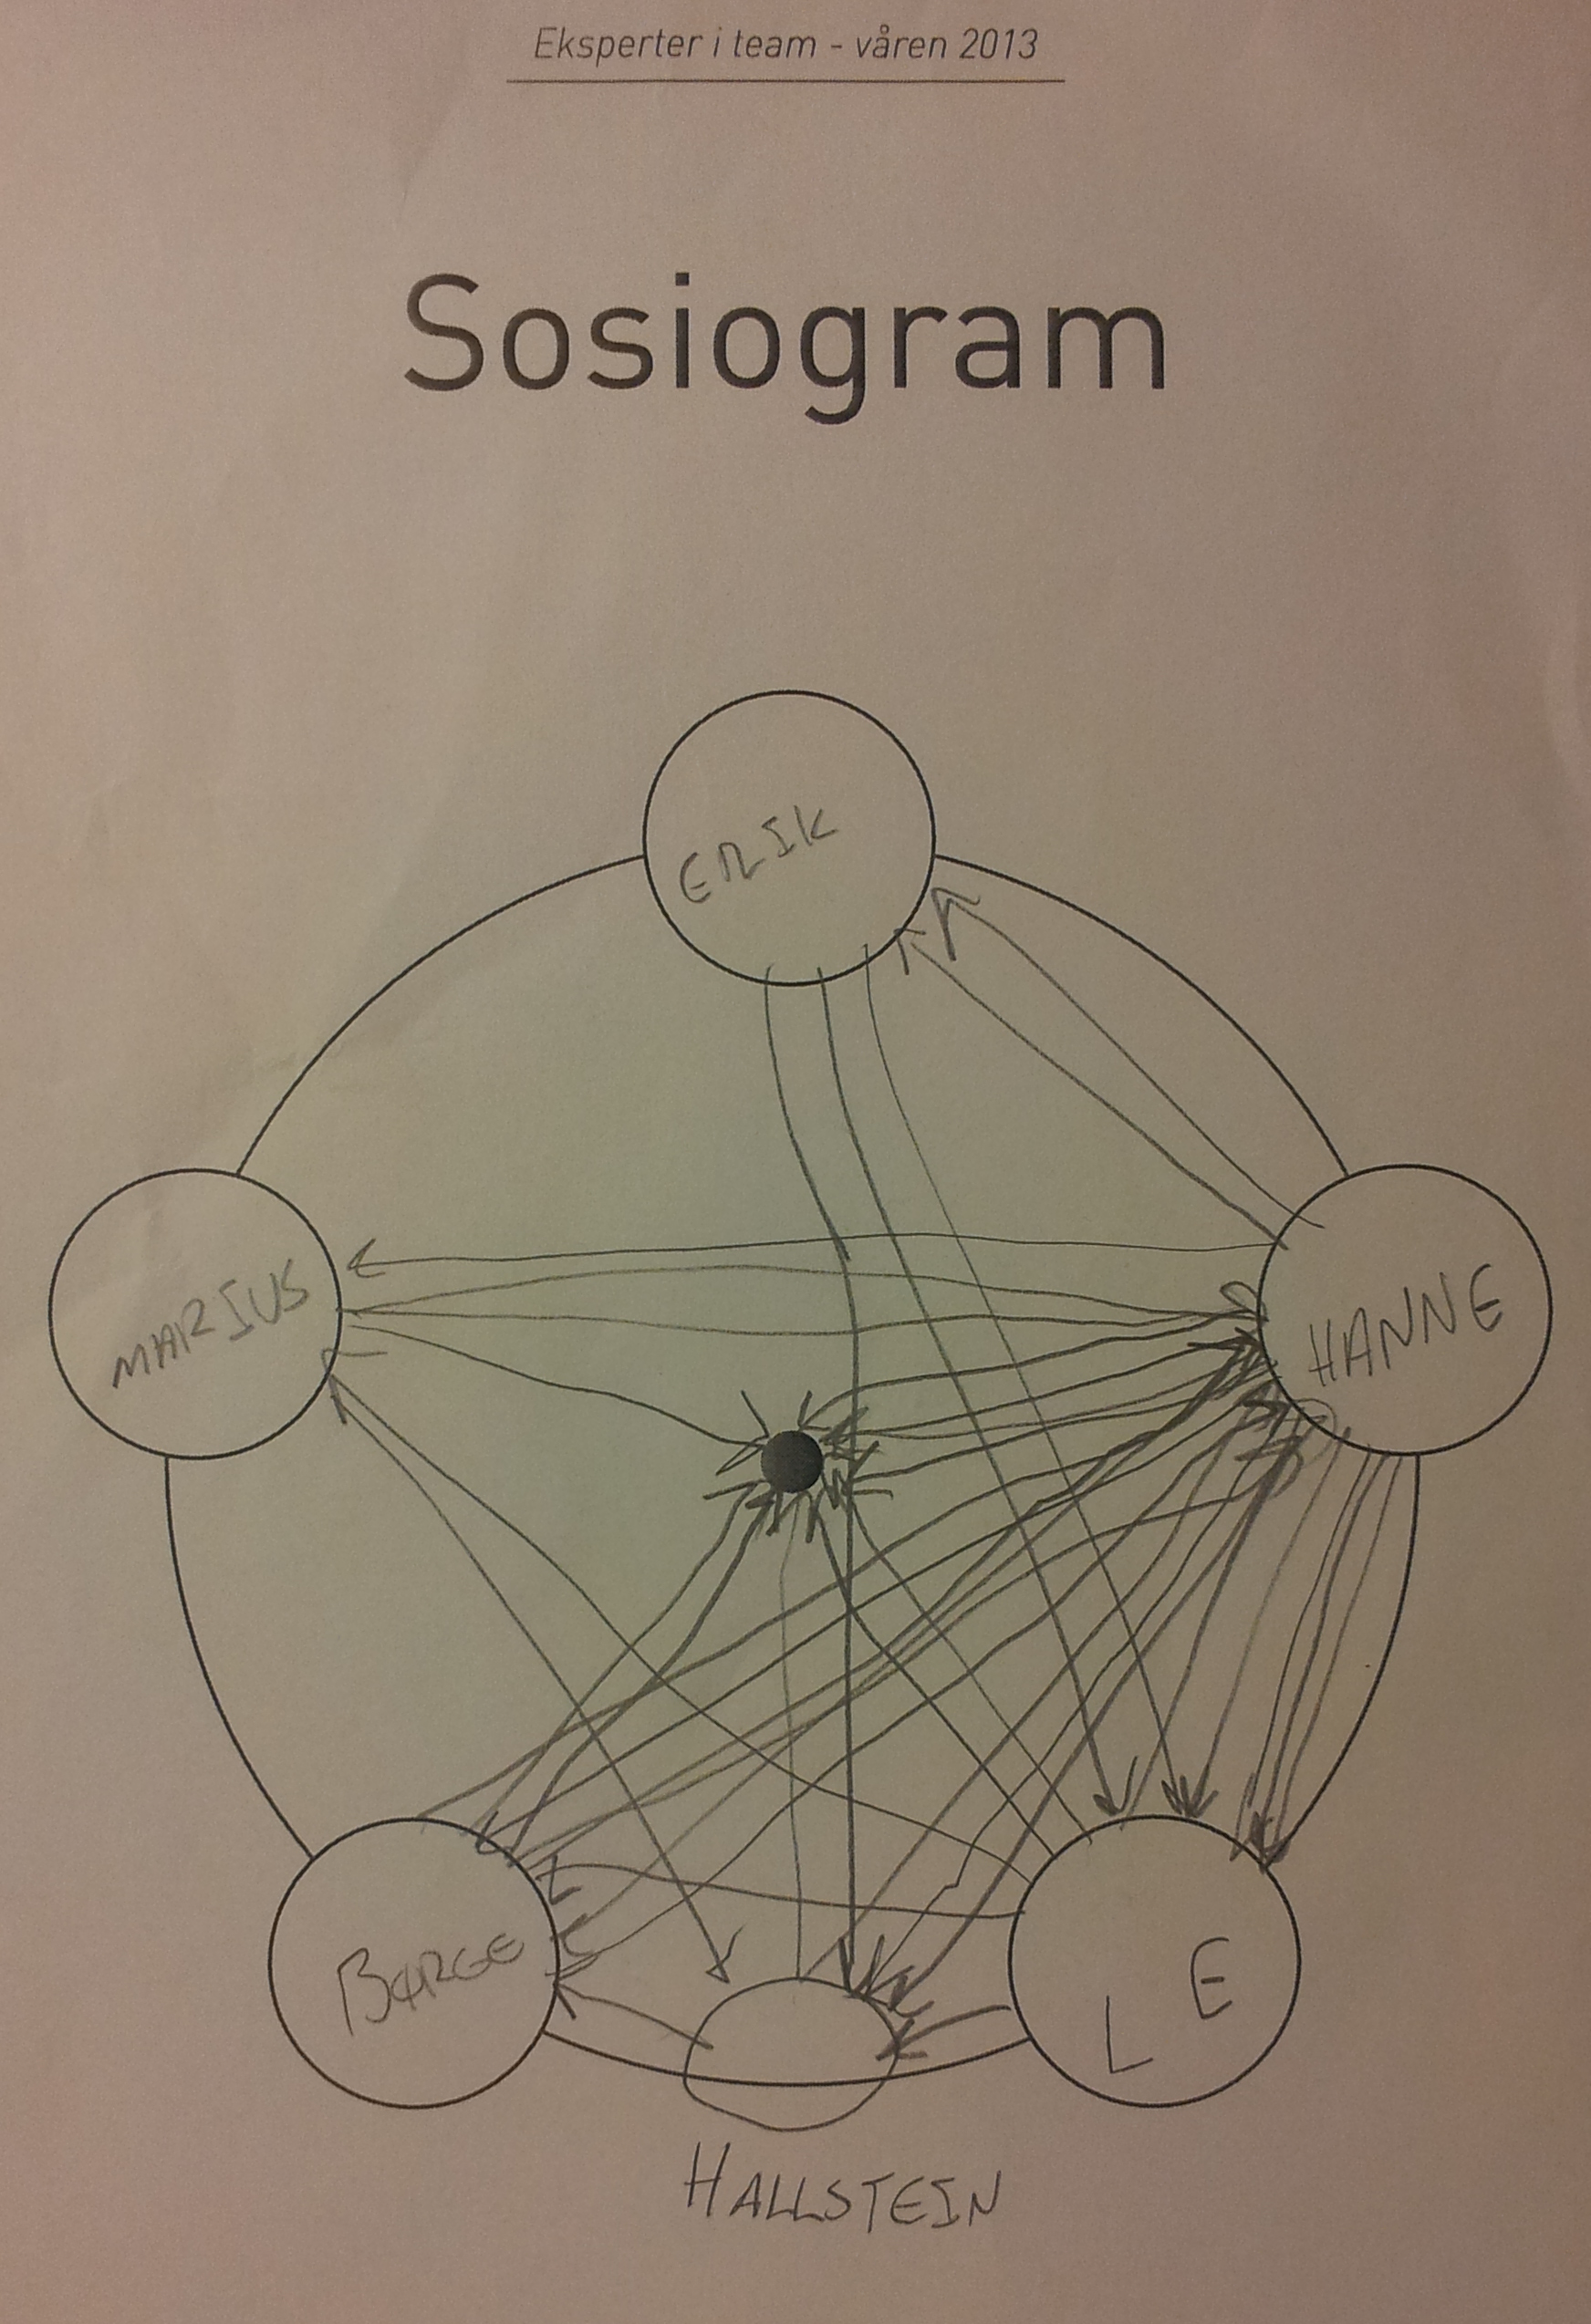
\includegraphics[width=0.7\textwidth]{Figures/sosiogram.png}}
	\end{center}
	\caption[The Sosiogram]{The Sosiogram we got from the facilitators after they observed a discussion in the group}
	\label{fig:sosiogram}
\end{figure}